% Graphic for TeX using PGF
% Title: S:\Senior Project\seniorProject2-2020-21-Docs\figs\dia\systemOperationFlowchart.dia
% Creator: Dia v0.97.2
% CreationDate: Tue Dec 01 10:16:03 2020
% For: Jason Braker
% \usepackage{tikz}
% The following commands are not supported in PSTricks at present
% We define them conditionally, so when they are implemented,
% this pgf file will use them.
\ifx\du\undefined
  \newlength{\du}
\fi
\setlength{\du}{15\unitlength}
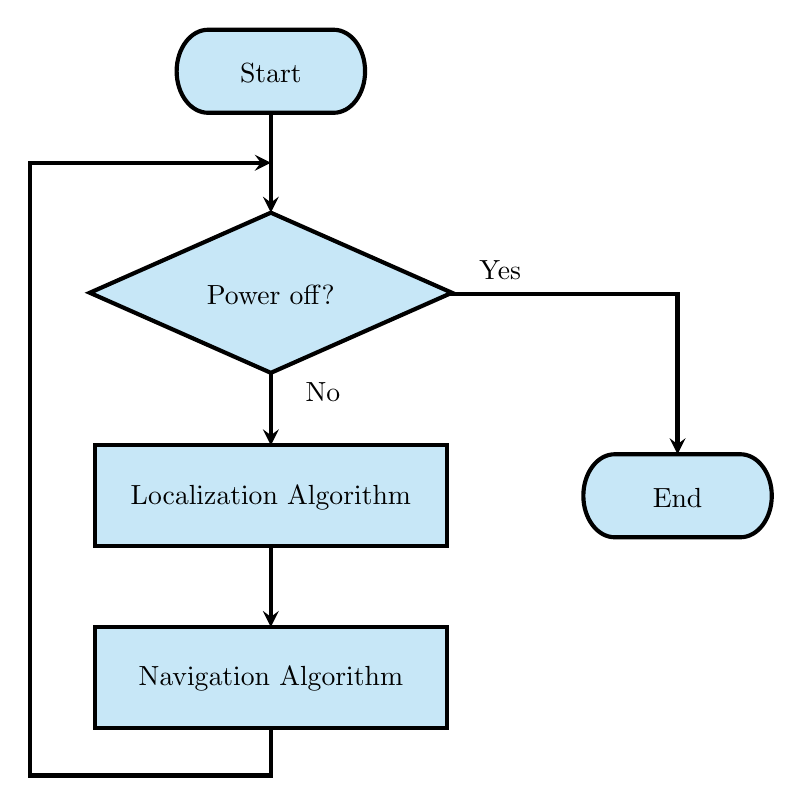
\begin{tikzpicture}
\pgftransformxscale{1.000000}
\pgftransformyscale{-1.000000}
\definecolor{dialinecolor}{rgb}{0.000000, 0.000000, 0.000000}
\pgfsetstrokecolor{dialinecolor}
\definecolor{dialinecolor}{rgb}{1.000000, 1.000000, 1.000000}
\pgfsetfillcolor{dialinecolor}
\pgfsetlinewidth{0.100000\du}
\pgfsetdash{}{0pt}
\pgfsetdash{}{0pt}
\pgfsetbuttcap
\pgfsetmiterjoin
\pgfsetlinewidth{0.100000\du}
\pgfsetbuttcap
\pgfsetmiterjoin
\pgfsetdash{}{0pt}
\definecolor{dialinecolor}{rgb}{0.780392, 0.905882, 0.968627}
\pgfsetfillcolor{dialinecolor}
\pgfpathmoveto{\pgfpoint{22.956985\du}{4.485160\du}}
\pgfpathlineto{\pgfpoint{25.983235\du}{4.485160\du}}
\pgfpathcurveto{\pgfpoint{26.401073\du}{4.485160\du}}{\pgfpoint{26.739798\du}{4.932875\du}}{\pgfpoint{26.739798\du}{5.485160\du}}
\pgfpathcurveto{\pgfpoint{26.739798\du}{6.037445\du}}{\pgfpoint{26.401073\du}{6.485160\du}}{\pgfpoint{25.983235\du}{6.485160\du}}
\pgfpathlineto{\pgfpoint{22.956985\du}{6.485160\du}}
\pgfpathcurveto{\pgfpoint{22.539147\du}{6.485160\du}}{\pgfpoint{22.200423\du}{6.037445\du}}{\pgfpoint{22.200423\du}{5.485160\du}}
\pgfpathcurveto{\pgfpoint{22.200423\du}{4.932875\du}}{\pgfpoint{22.539147\du}{4.485160\du}}{\pgfpoint{22.956985\du}{4.485160\du}}
\pgfusepath{fill}
\definecolor{dialinecolor}{rgb}{0.000000, 0.000000, 0.000000}
\pgfsetstrokecolor{dialinecolor}
\pgfpathmoveto{\pgfpoint{22.956985\du}{4.485160\du}}
\pgfpathlineto{\pgfpoint{25.983235\du}{4.485160\du}}
\pgfpathcurveto{\pgfpoint{26.401073\du}{4.485160\du}}{\pgfpoint{26.739798\du}{4.932875\du}}{\pgfpoint{26.739798\du}{5.485160\du}}
\pgfpathcurveto{\pgfpoint{26.739798\du}{6.037445\du}}{\pgfpoint{26.401073\du}{6.485160\du}}{\pgfpoint{25.983235\du}{6.485160\du}}
\pgfpathlineto{\pgfpoint{22.956985\du}{6.485160\du}}
\pgfpathcurveto{\pgfpoint{22.539147\du}{6.485160\du}}{\pgfpoint{22.200423\du}{6.037445\du}}{\pgfpoint{22.200423\du}{5.485160\du}}
\pgfpathcurveto{\pgfpoint{22.200423\du}{4.932875\du}}{\pgfpoint{22.539147\du}{4.485160\du}}{\pgfpoint{22.956985\du}{4.485160\du}}
\pgfusepath{stroke}
% setfont left to latex
\definecolor{dialinecolor}{rgb}{0.000000, 0.000000, 0.000000}
\pgfsetstrokecolor{dialinecolor}
\node at (24.470110\du,5.525160\du){Start};
\pgfsetlinewidth{0.100000\du}
\pgfsetdash{}{0pt}
\pgfsetdash{}{0pt}
\pgfsetbuttcap
{
\definecolor{dialinecolor}{rgb}{0.000000, 0.000000, 0.000000}
\pgfsetfillcolor{dialinecolor}
% was here!!!
\pgfsetarrowsend{stealth}
\definecolor{dialinecolor}{rgb}{0.000000, 0.000000, 0.000000}
\pgfsetstrokecolor{dialinecolor}
\draw (24.470110\du,12.750000\du)--(24.470110\du,14.497300\du);
}
\pgfsetlinewidth{0.100000\du}
\pgfsetdash{}{0pt}
\pgfsetdash{}{0pt}
\pgfsetbuttcap
{
\definecolor{dialinecolor}{rgb}{0.000000, 0.000000, 0.000000}
\pgfsetfillcolor{dialinecolor}
% was here!!!
\pgfsetarrowsend{stealth}
\definecolor{dialinecolor}{rgb}{0.000000, 0.000000, 0.000000}
\pgfsetstrokecolor{dialinecolor}
\draw (24.470110\du,6.485160\du)--(24.470110\du,8.891790\du);
}
\pgfsetlinewidth{0.100000\du}
\pgfsetdash{}{0pt}
\pgfsetdash{}{0pt}
\pgfsetmiterjoin
\pgfsetbuttcap
{
\definecolor{dialinecolor}{rgb}{0.000000, 0.000000, 0.000000}
\pgfsetfillcolor{dialinecolor}
% was here!!!
\pgfsetarrowsend{stealth}
{\pgfsetcornersarced{\pgfpoint{0.000000\du}{0.000000\du}}\definecolor{dialinecolor}{rgb}{0.000000, 0.000000, 0.000000}
\pgfsetstrokecolor{dialinecolor}
\draw (24.470110\du,21.300000\du)--(24.470110\du,22.450000\du)--(18.662000\du,22.450000\du)--(18.662000\du,7.688470\du)--(24.470100\du,7.688470\du);
}}
\pgfsetlinewidth{0.100000\du}
\pgfsetdash{}{0pt}
\pgfsetdash{}{0pt}
\pgfsetmiterjoin
\pgfsetbuttcap
{
\definecolor{dialinecolor}{rgb}{0.000000, 0.000000, 0.000000}
\pgfsetfillcolor{dialinecolor}
% was here!!!
\pgfsetarrowsend{stealth}
{\pgfsetcornersarced{\pgfpoint{0.000000\du}{0.000000\du}}\definecolor{dialinecolor}{rgb}{0.000000, 0.000000, 0.000000}
\pgfsetstrokecolor{dialinecolor}
\draw (28.832020\du,10.820895\du)--(28.832020\du,10.850000\du)--(34.267610\du,10.850000\du)--(34.267610\du,14.711150\du);
}}
% setfont left to latex
\definecolor{dialinecolor}{rgb}{0.000000, 0.000000, 0.000000}
\pgfsetstrokecolor{dialinecolor}
\node[anchor=west] at (29.220400\du,10.266000\du){Yes};
% setfont left to latex
\definecolor{dialinecolor}{rgb}{0.000000, 0.000000, 0.000000}
\pgfsetstrokecolor{dialinecolor}
\node[anchor=west] at (25.033800\du,13.204600\du){No};
\definecolor{dialinecolor}{rgb}{0.780392, 0.905882, 0.968627}
\pgfsetfillcolor{dialinecolor}
\fill (20.230576\du,18.872300\du)--(20.230576\du,21.300000\du)--(28.709644\du,21.300000\du)--(28.709644\du,18.872300\du)--cycle;
\pgfsetlinewidth{0.100000\du}
\pgfsetdash{}{0pt}
\pgfsetdash{}{0pt}
\pgfsetmiterjoin
\definecolor{dialinecolor}{rgb}{0.000000, 0.000000, 0.000000}
\pgfsetstrokecolor{dialinecolor}
\draw (20.230576\du,18.872300\du)--(20.230576\du,21.300000\du)--(28.709644\du,21.300000\du)--(28.709644\du,18.872300\du)--cycle;
% setfont left to latex
\definecolor{dialinecolor}{rgb}{0.000000, 0.000000, 0.000000}
\pgfsetstrokecolor{dialinecolor}
\node at (24.470110\du,20.126150\du){Navigation Algorithm};
\definecolor{dialinecolor}{rgb}{0.780392, 0.905882, 0.968627}
\pgfsetfillcolor{dialinecolor}
\fill (24.470110\du,8.891790\du)--(28.832020\du,10.820895\du)--(24.470110\du,12.750000\du)--(20.108200\du,10.820895\du)--cycle;
\pgfsetlinewidth{0.100000\du}
\pgfsetdash{}{0pt}
\pgfsetdash{}{0pt}
\pgfsetmiterjoin
\definecolor{dialinecolor}{rgb}{0.000000, 0.000000, 0.000000}
\pgfsetstrokecolor{dialinecolor}
\draw (24.470110\du,8.891790\du)--(28.832020\du,10.820895\du)--(24.470110\du,12.750000\du)--(20.108200\du,10.820895\du)--cycle;
% setfont left to latex
\definecolor{dialinecolor}{rgb}{0.000000, 0.000000, 0.000000}
\pgfsetstrokecolor{dialinecolor}
\node at (24.470110\du,10.860895\du){Power off?};
\pgfsetlinewidth{0.100000\du}
\pgfsetdash{}{0pt}
\pgfsetdash{}{0pt}
\pgfsetbuttcap
{
\definecolor{dialinecolor}{rgb}{0.000000, 0.000000, 0.000000}
\pgfsetfillcolor{dialinecolor}
% was here!!!
\pgfsetarrowsend{stealth}
\definecolor{dialinecolor}{rgb}{0.000000, 0.000000, 0.000000}
\pgfsetstrokecolor{dialinecolor}
\draw (24.470110\du,16.925000\du)--(24.470110\du,18.872300\du);
}
\definecolor{dialinecolor}{rgb}{0.780392, 0.905882, 0.968627}
\pgfsetfillcolor{dialinecolor}
\fill (20.230576\du,14.497300\du)--(20.230576\du,16.925000\du)--(28.709644\du,16.925000\du)--(28.709644\du,14.497300\du)--cycle;
\pgfsetlinewidth{0.100000\du}
\pgfsetdash{}{0pt}
\pgfsetdash{}{0pt}
\pgfsetmiterjoin
\definecolor{dialinecolor}{rgb}{0.000000, 0.000000, 0.000000}
\pgfsetstrokecolor{dialinecolor}
\draw (20.230576\du,14.497300\du)--(20.230576\du,16.925000\du)--(28.709644\du,16.925000\du)--(28.709644\du,14.497300\du)--cycle;
% setfont left to latex
\definecolor{dialinecolor}{rgb}{0.000000, 0.000000, 0.000000}
\pgfsetstrokecolor{dialinecolor}
\node at (24.470110\du,15.751150\du){Localization Algorithm};
\pgfsetlinewidth{0.100000\du}
\pgfsetdash{}{0pt}
\pgfsetdash{}{0pt}
\pgfsetbuttcap
\pgfsetmiterjoin
\pgfsetlinewidth{0.100000\du}
\pgfsetbuttcap
\pgfsetmiterjoin
\pgfsetdash{}{0pt}
\definecolor{dialinecolor}{rgb}{0.780392, 0.905882, 0.968627}
\pgfsetfillcolor{dialinecolor}
\pgfpathmoveto{\pgfpoint{32.754485\du}{14.711150\du}}
\pgfpathlineto{\pgfpoint{35.780735\du}{14.711150\du}}
\pgfpathcurveto{\pgfpoint{36.198573\du}{14.711150\du}}{\pgfpoint{36.537298\du}{15.158865\du}}{\pgfpoint{36.537298\du}{15.711150\du}}
\pgfpathcurveto{\pgfpoint{36.537298\du}{16.263435\du}}{\pgfpoint{36.198573\du}{16.711150\du}}{\pgfpoint{35.780735\du}{16.711150\du}}
\pgfpathlineto{\pgfpoint{32.754485\du}{16.711150\du}}
\pgfpathcurveto{\pgfpoint{32.336647\du}{16.711150\du}}{\pgfpoint{31.997923\du}{16.263435\du}}{\pgfpoint{31.997923\du}{15.711150\du}}
\pgfpathcurveto{\pgfpoint{31.997923\du}{15.158865\du}}{\pgfpoint{32.336647\du}{14.711150\du}}{\pgfpoint{32.754485\du}{14.711150\du}}
\pgfusepath{fill}
\definecolor{dialinecolor}{rgb}{0.000000, 0.000000, 0.000000}
\pgfsetstrokecolor{dialinecolor}
\pgfpathmoveto{\pgfpoint{32.754485\du}{14.711150\du}}
\pgfpathlineto{\pgfpoint{35.780735\du}{14.711150\du}}
\pgfpathcurveto{\pgfpoint{36.198573\du}{14.711150\du}}{\pgfpoint{36.537298\du}{15.158865\du}}{\pgfpoint{36.537298\du}{15.711150\du}}
\pgfpathcurveto{\pgfpoint{36.537298\du}{16.263435\du}}{\pgfpoint{36.198573\du}{16.711150\du}}{\pgfpoint{35.780735\du}{16.711150\du}}
\pgfpathlineto{\pgfpoint{32.754485\du}{16.711150\du}}
\pgfpathcurveto{\pgfpoint{32.336647\du}{16.711150\du}}{\pgfpoint{31.997923\du}{16.263435\du}}{\pgfpoint{31.997923\du}{15.711150\du}}
\pgfpathcurveto{\pgfpoint{31.997923\du}{15.158865\du}}{\pgfpoint{32.336647\du}{14.711150\du}}{\pgfpoint{32.754485\du}{14.711150\du}}
\pgfusepath{stroke}
% setfont left to latex
\definecolor{dialinecolor}{rgb}{0.000000, 0.000000, 0.000000}
\pgfsetstrokecolor{dialinecolor}
\node at (34.267610\du,15.751150\du){End};
\end{tikzpicture}
